\todo{todo}
to mention:
google app engine
android stuff, api for graphs, others?
arduino code detail?


The software consist of three components. The device on the bin, one cloudservice and one android client.
The components interact using the client-server model over the web, in a cloud-based architecture (figure ~\ref{fig:architecture}).

\begin{figure}
\centering
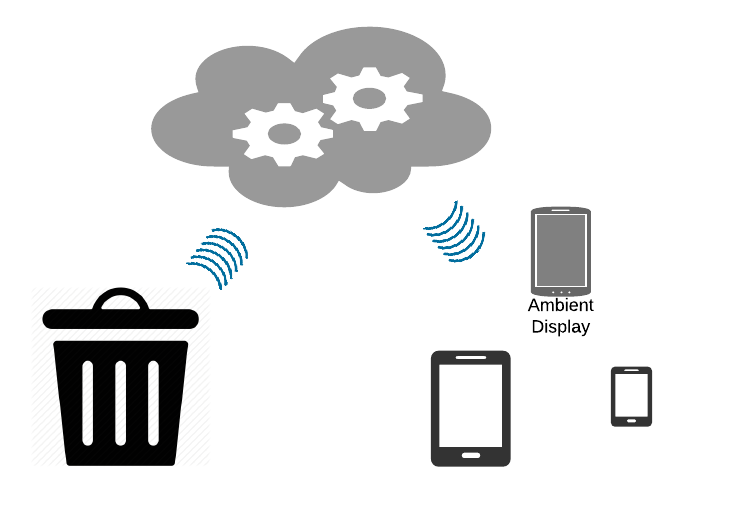
\includegraphics[scale=.6]{img/architecture}
\caption{Cloud-based architecture}
\label{fig:architecture}
\end{figure}

\begin{figure}
\centering
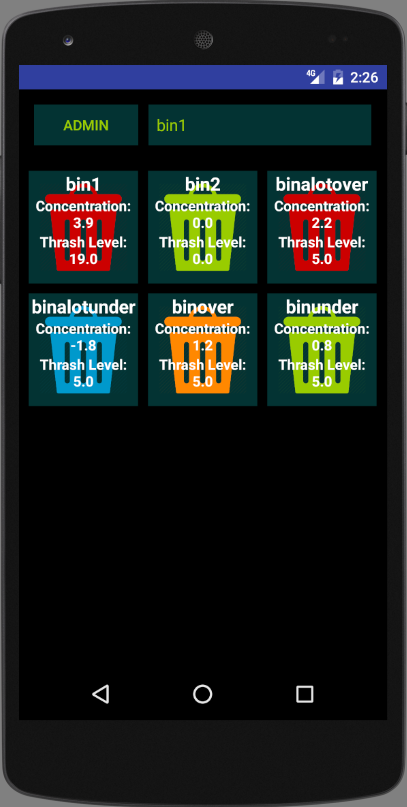
\includegraphics[scale=.3]{img/screen_admin}
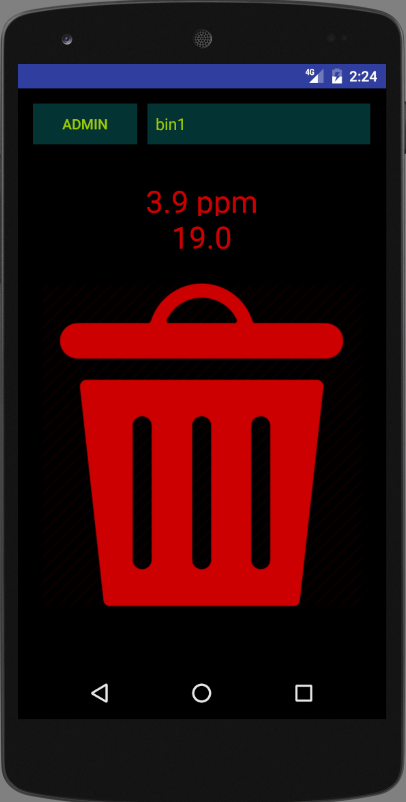
\includegraphics[scale=.3]{img/screen_single}
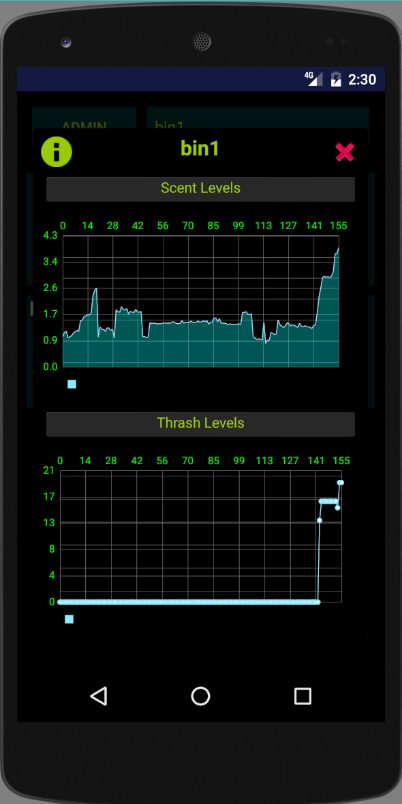
\includegraphics[scale=.3]{img/screen_stats}
\caption{Image of the three main views in the android client} 	
\label{fig:clientmodes}
\end{figure}

\begin{figure}
\centering
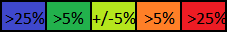
\includegraphics{img/app_colors_nb}
\caption{Image of the color codes ranging, from deviation under the norm to deviation over the norm} 
\label{fig:colorcodes}
\end{figure}

On the \textbf{bin}, the gas sensor first needs to go through a warm-up period of about 15-20 minutes, during which the sensor is energised. The resistance registered by the sensor drops sharply for the first minutes after energising, regardless of the presence of gases. This behaviour is commonly known as \textit{Initial Action}, and could cause a system to mistakenly report presence of gases during the first minutes of activity\cite{tgs2602}.

After the warm-up period, the system will go through a period of \textit{calibration} (5 minutes), during which the value Ro (resistance measured by the gas sensor in clean air) is computed as an average of 300 samples.
During this period the sensor has to be kept in "clean air", or  in an environment considered to be in a base condition, because later measurements will rely on this value.

After warm up and calibration, the gas concentration sensed by the sensor will be in the form of a ratio \textit{Rs/Ro}, where Rs is the resistance measured by the sensor at a given time and Ro is the constant value detected in clean air.
This means that if the gas concentrations perceived by the sensor are very similar as the ones in clean air, the ratio will be close to 1.
The more the values Rs and Ro differ, the more far from 1 the ratio will be.

The android client can provide statistics about different smartbins - it only supports  presentation of data in its current form.
It supports two modes: \textbf{Admin mode} and \textbf{Single Bin mode}.
Admin mode includes overview of every single bin and graphs for each bin. The graphs are only available as long as enough context information is present see figure~\ref{fig:clientmodes}.

 Single bin mode provides a view of the current bin state.
 
 The bin state is divided into five different categories, this is represented visually as colors.
 The order is, \textit{blue}, \textit{dark green}, \textit{green}, \textit{orange}, and \textit{red}, as seen on figure~\ref{fig:colorcodes}.
The middle one, \textit{green}, is when the concentration is deviating with at most 5\%, next tier \textit{dark green} and \textit{orange} is a deviation of at most 25\%, and the last ones \textit{blue} and \textit{red} are deviations above 25\%.